% !TEX root = ./memoire/main.tex

\chapter{Introduction}

\section{Contexte Industriel}

Dans le domaine de la production d'énergie électrique, l'énergie nucléaire est une source d'énergie qui s'est imposée à de nombreux pays industrialisés. En 2023, l'industrie électronucléaire a représenté 65\% de la production totale d'électricité en France, avec un parc composé de 56 réacteurs à eau pressurisée (REP) répartis sur 18 centrales~\cite{rte2023}. Dans le monde, la production nucléaire ne fait qu'augmenter. Fin 2022, la capacité totale des 438 réacteurs nucléaires de puissance en exploitation dans 32 pays s’établissait à 393,8 gigawatts électriques (GWe). Si aujourd'hui, le nucléaire représente près de 9,8\% de la production mondiale, elle pourrait attendre 14\% du bouquet électrique en 2050. D'ici 2035, le nombre de pays qui exploitent des centrales nucléaires pourrait augmenter de quelque 30\%~\cite{aiea2023}. Le secteur est également en constante mutation avec le développement de réacteurs de IV\textsubscript{ème} génération ou des SMR (\textit{Small Modular Reactor})~\cite{academie2022}. Si ce secteur attire, c'est en particulier car il offre un très bon rapport qualité prix et est faiblement émettrice en gaz à effet de serre. Son facteur d'émission, c'est à dire la quantité d'émissions de gaz à effet de serre par unité d'énergie produite, est estimé à 12g eq$CO2$/kWh~\cite{schlomer_technology-specific_nodate}. Il serait même encore plus faible en France avec 4g eq$CO2$/kWh~\cite{edf2022}. Ainsi elle est aussi émettrice que l'éolien ou bien la production photovoltaïque et est 100 à 1000 fois moins émettrice que les centrales à énergie fossiles.

L'urgence climatique pousse à considérer l'énergie nucléaire comme un levier essentiel dans la transition énergétique, offrant une alternative viable aux énergies fossiles. Cependant, cette option soulève une série de préoccupations. Outre les inquiétudes liées à la sécurité des installations et au risque de prolifération nucléaire~\cite{npt_resolution}, il est crucial d'aborder la question des déchets hautement radioactifs générés tout au long du fonctionnement des réacteurs. Chaque année, la production d'électricité entraîne la création de près de 2 kg de déchets par habitant. Une infime proportion constitue les déchets à vie longue, mais ils représentent la majorité de l'activité radioactive (0.2\% des stocks pour 95\% de l'activité). En outre, il est impératif de préserver les réserves de combustible nucléaire. Dans cette optique, les avancées technologiques telles que les réacteurs de quatrième génération visent à optimiser l'utilisation des ressources en transmutant l'uranium 238 en plutonium 239. Ainsi, la question du retraitement et de la fermeture du cycle nucléaire reste cruciale (Figure~\ref{fig:cycle_comb}).

\begin{figure}
    \centering
    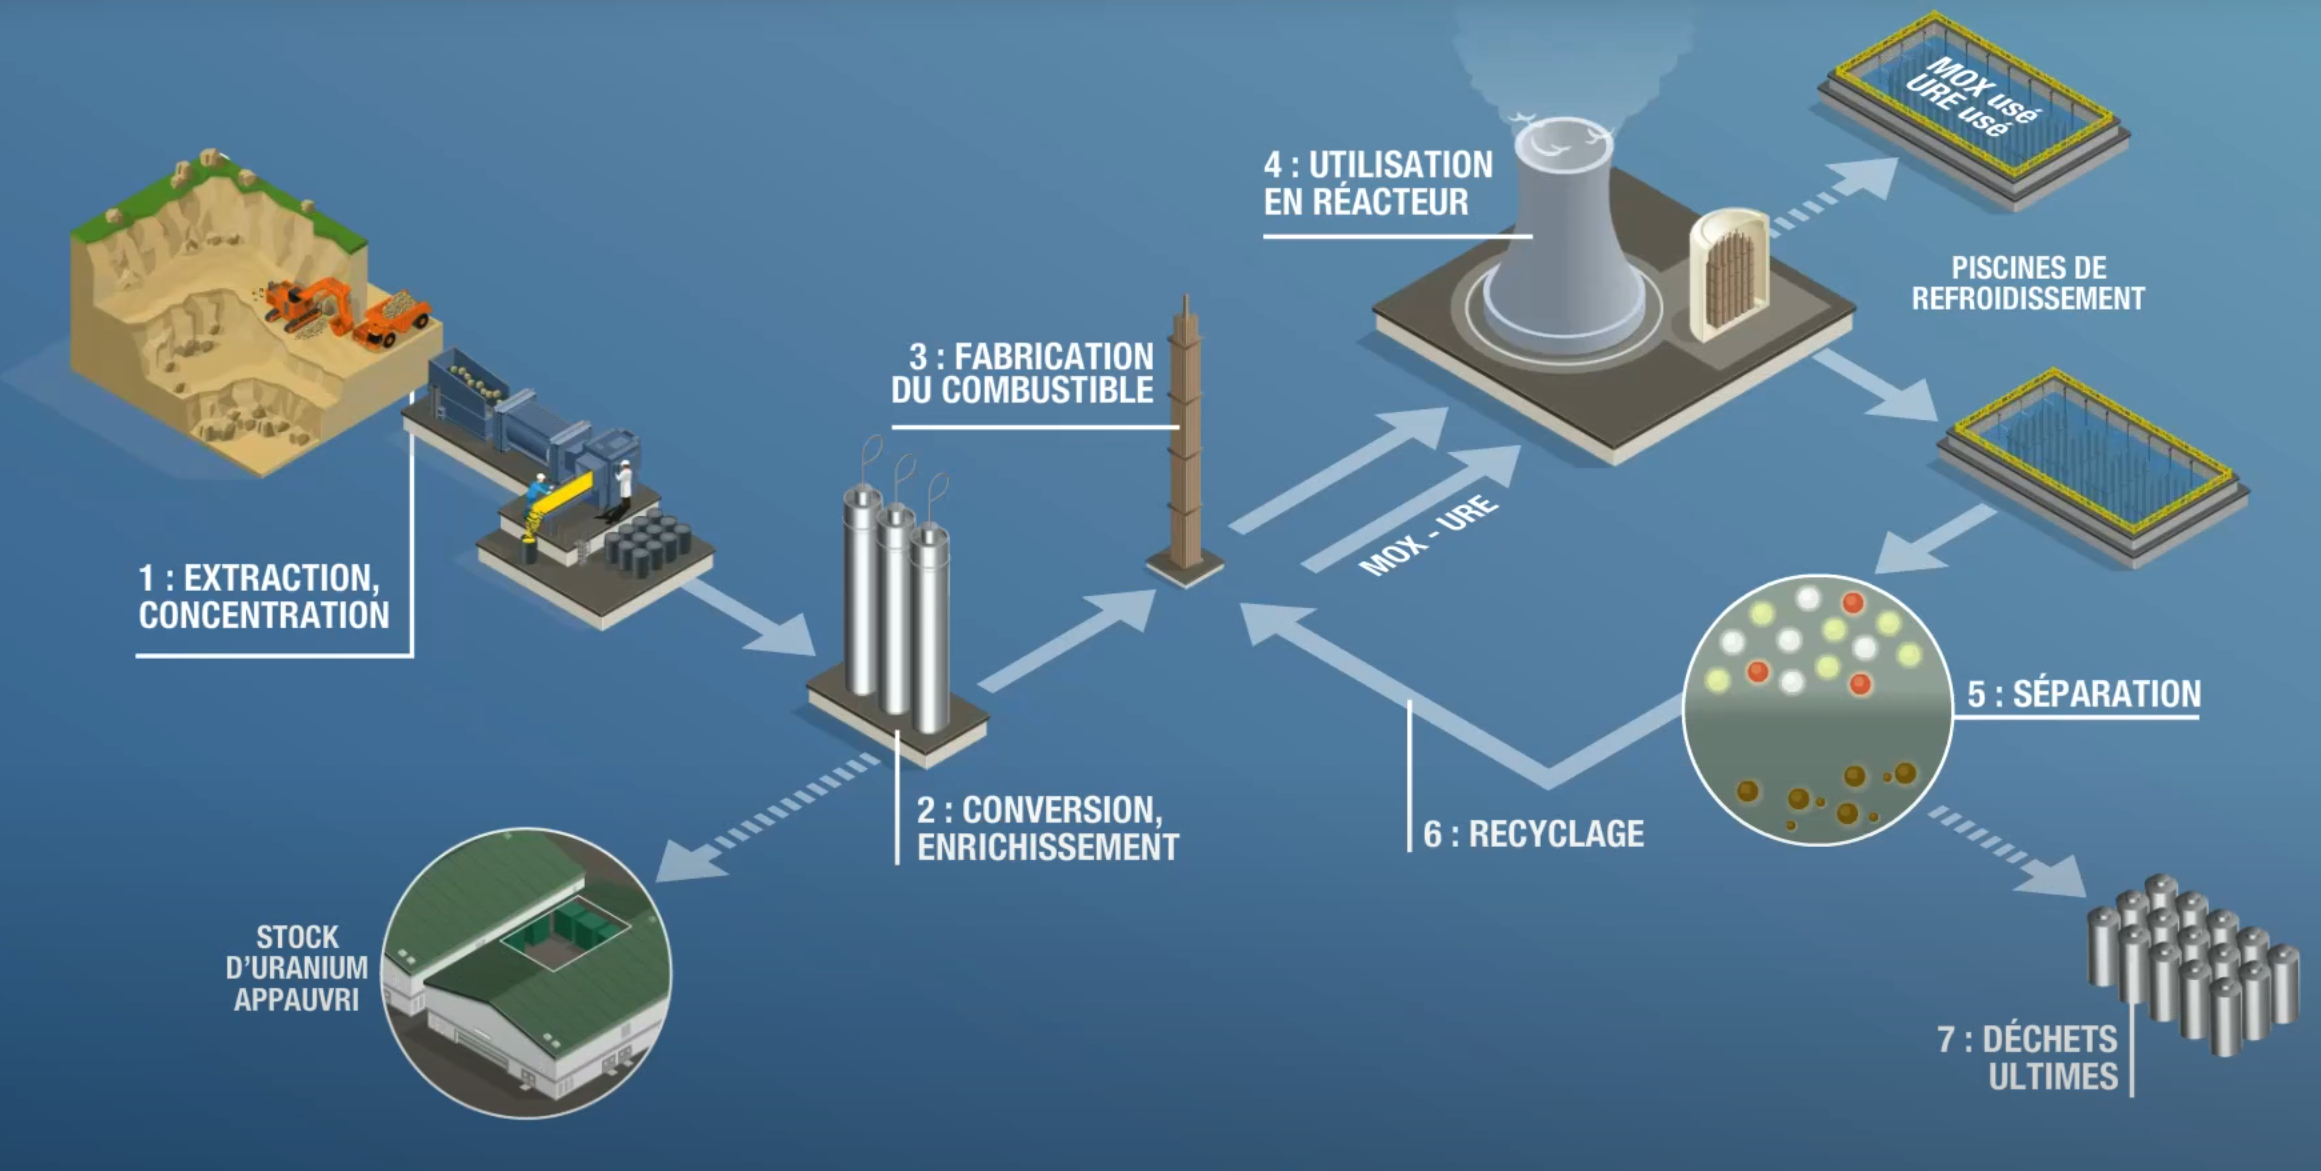
\includegraphics[width=0.8\textwidth]{cycle.png}%Le cycle du combustible nucléaire © CEACom Ci Com Cacycle-combustible-nucleaire.jpg}
    \caption{Représentation du cycle du combustible nucléaire. La fermeture du cycle passe par un recyclage en aval du cycle. \copyright CEA/Com Ci Com Ca}~\label{fig:cycle_comb}
\end{figure}

C'est dans cette perspective que le combustible MOX (Mélange d’OXyde de plutonium et d’OXyde d’uranium) a été développé afin de recycler une partie des matières nucléaires issues du traitement des combustibles à Uranium Naturel Enrichi (UNE). Le combustible nucléaire est généralement composé de dioxyde d'uranium (UO2), enrichi à 3-5\% en uranium 235. Le combustible MOX (\textit{Mixed Oxide}) combinant dioxyde de plutonium (PuO2) et dioxyde d'uranium (UO2) est particulièrement utile pour les réacteurs à neutrons rapides, mais peut également être employé dans les réacteurs à eau pressurisée actuels.
% La teneur en PuO2 dans le MOX varie entre 8\% et 30\%, en fonction des besoins spécifiques du réacteur. Le PuO2 provient du recyclage dans les usines de retraitement, car le plutonium est un produit de fission de l'uranium 235. Ces deux oxydes diffèrent par leurs propriétés, notamment leur surface spécifique, avec 2 m²/g pour UO2 et 6 m²/g pour PuO2. En termes de morphologie, les particules d'UO2 forment des agglomérats, tandis que le PuO2 présente des plaquettes submicroniques.
Tout comme le combustible à base d'uranium, le combustible est présent dans les réacteurs sous forme de pastille cylindrique de diamètre et de hauteur d'environ 1 cm. Elles sont ensuite empilées dans des gaines métallique et constitues un élément de crayon d'environ 4 m de haut. Ces éléments sont ensuite réuni dans un assemblage dans une grille de près de 250 éléments. Pour obtenir ces pastilles, la fabrications passe par différentes étapes de fabrication, illustrées en Figure~\ref{fig:fab_comb} en particulier une phase de mélange et de broyage qui a lieu au sein d'un broyeur à boulets comme illustré

\begin{figure}[h]
    \centering
    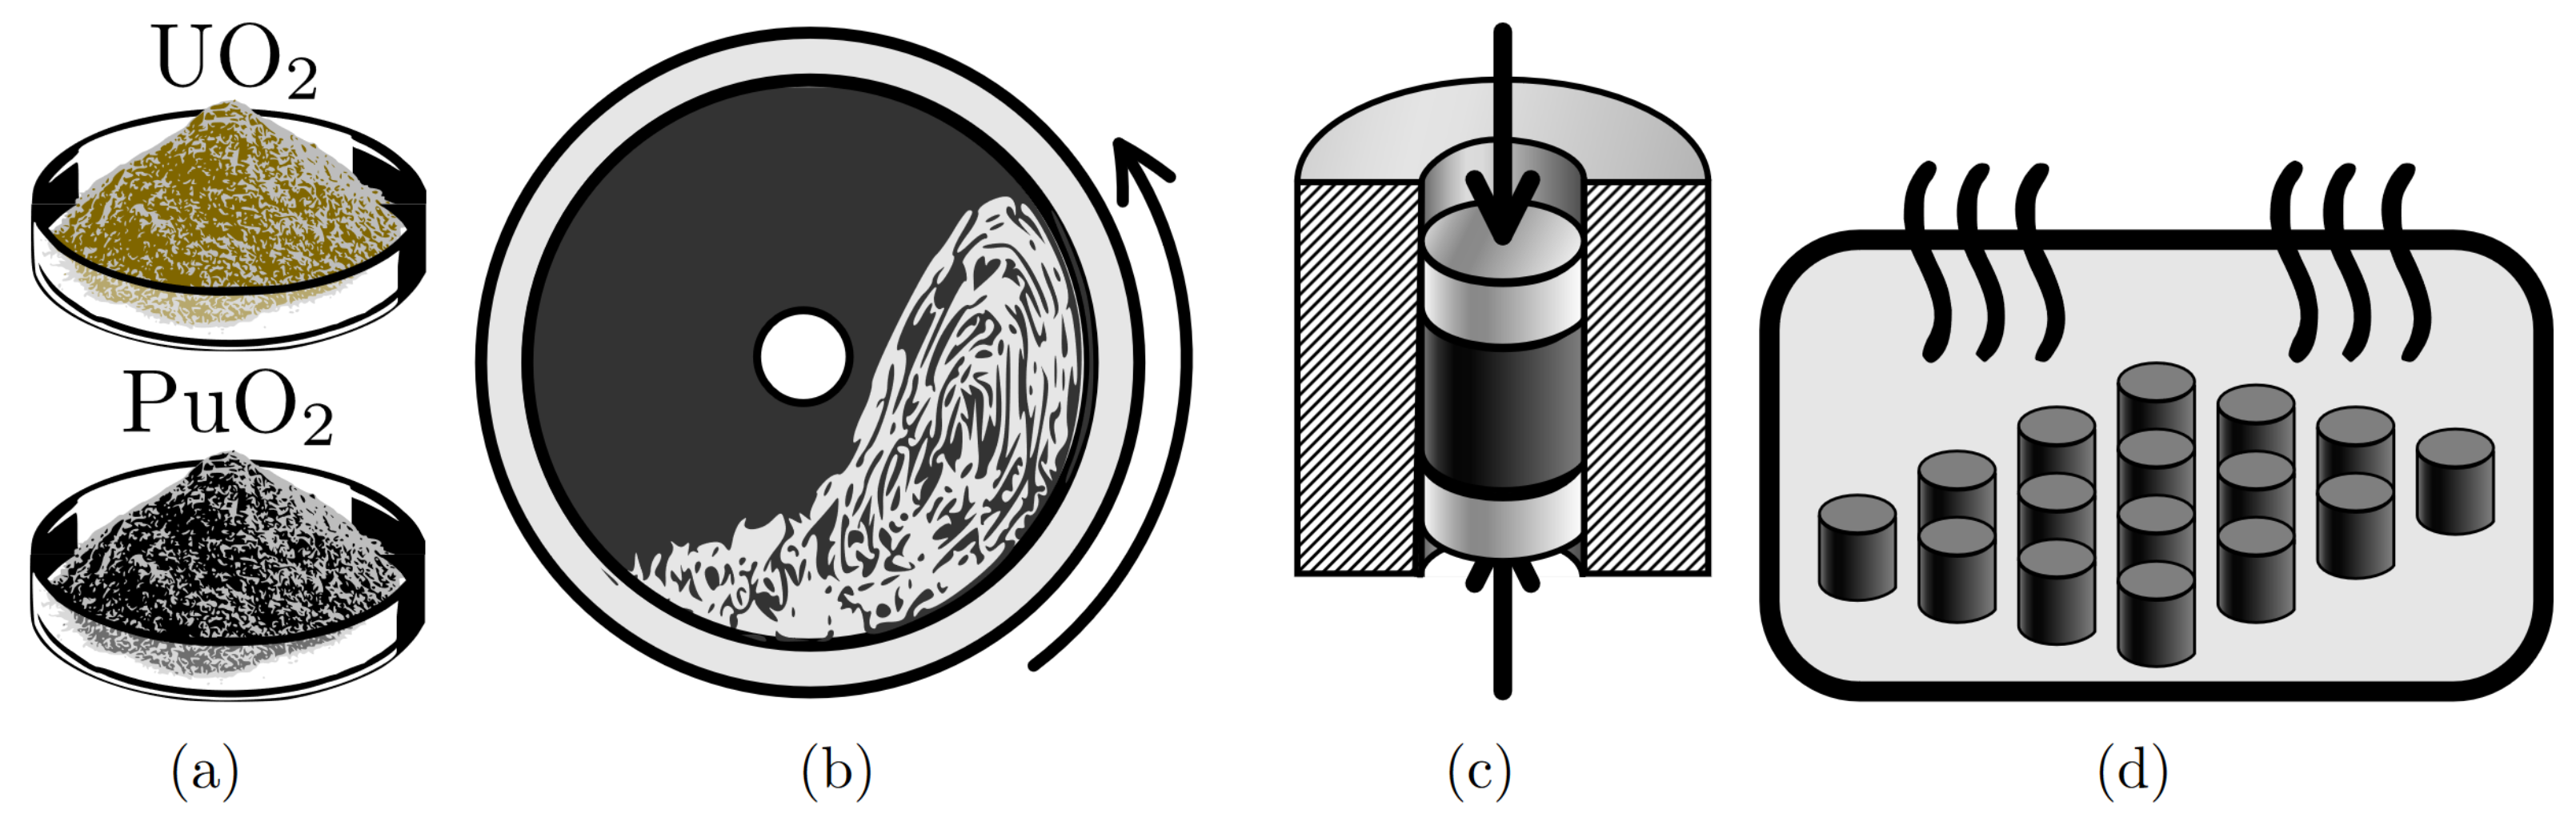
\includegraphics[width=\textwidth]{fuel_manufacturing.png}
    \caption{Les principales étapes de la fabrication des pastilles de MOX sont : (a) les matières premières, (b) le mélange des poudres, (c) la mise en forme des pastilles et (d) le frittage.}~\label{fig:fab_comb}
\end{figure}

Ce dispositif cylindrique, rempli de boules de broyage, appelés corps broyants, met en oeuvre un processus de rotation pour broyer finement le mélange de poudres d'oxyde. Cette étape dure entre 2 et 4h et qui va permettre de mélanger les deux poudres afin d'avoir un mélange homogène à une granulométrie moyenne de $5\mu m$. En effet il est nécessaire d'avoir une poudre fine afin d'obtenir une bonne coulabilité de poudre. Cette propriété est déterminante tout au long de la fabrication et particulièrement pour permettre la mise en forme des pastilles~\cite{ABE2012393}. D'autre part, cette étape est déterminante pour éviter d'avoir des haute concentration de Pu, à l'origine de points chauds ou du relâchement de gaz de fission, tout deux facteurs d'accident dans le réacteur~\cite{BOULORE201579, oudinet2015}.

Cependant, le contrôle de cette étape de mélange et de broyage est déterminé de manière empirique par l'expérimentateur sur une variété de paramètres tels que la vitesse de rotation, le degré de remplissage, les proportions d'alimentation et de corps broyants. En effet, cette étape critique, assez simple dans son principe, reste encore mal comprise dans ses mécanismes physiques~\cite{Austin1981,Brandao2020,Mankosa1986,Datta2002,Capece2014}. C'est dans cette perspective que des outils complémentaires d'analyse sont nécessaires. Ainsi, des études expérimentales ont été mises en place. En particulier, la thèse de Giraud pour pouvoir déterminer des relations empirique entre les propriétés microscopiques du combustible MOX et du comportement rhéologique macroscopique du mélange~\cite{giraud_analyse_2020}. Ces études reposent sur des campagnes de mesures complexes nécessitant de la manipulation de poudres irradiées. L'environnements doit en particulier être scellé pour éviter la contamination. Les équipements sont spécialisés et exclusifs et un blindage est mis en place contre les radiations et la production de chaleur. De plus, les mesures effectuées sont soumises à des incertitudes et sont souvent spécifiques au problème.
D'autre part, des méthodes de simulation haute fidélité permettent de représenter le comportement des poudres. C'est en particulier la méthode des éléments discrets (DEM) qui a été utilisée dans les thèses de Orozco~\cite{Orozco2019} et Vu~\cite{vu_quasi-static_2023} pour simuler l'écoulement et les mécanismes de fragmentation au sein du tambour. Ces études ont permis en particulier de déterminer des grandeurs adimensionnelles pour pouvoir réaliser des changements d'échelle. Cependant il existe encore un écart substantiel entre les connaissances actuelles sur les mécanismes physiques régissant le processus de broyage et le besoin de modélisation prédictive et quantitative en vue des applications industrielles.

C'est dans cette optique que la construction d'un jumeau numérique est souhaitée afin d'améliorer la compréhension du procédé de mélange et de broyage ainsi que de d'optimiser le processus de broyage. Nous nous focaliserons dans ce travail uniquement sur la compréhension du mécanismes de mélange.



% L'objectif de notre travail est donc de développer un jumeau numérique afin de répondre à ces défis. Ce jumeau numérique permettra de combler le fossé entre les prédictions et les résultats réels, tout en optimisant l'utilisation des données disponibles pour améliorer les performances et l'efficacité du processus de broyage.